% !TEX TS-program = pdflatex
% !TEX encoding = UTF-8 Unicode

% This is a simple template for a LaTeX document using the "article" class.
% See "book", "report", "letter" for other types of document.

\documentclass[11pt]{article} % use larger type; default would be 10pt

\usepackage[utf8]{inputenc} % set input encoding (not needed with XeLaTeX)
\DeclareUnicodeCharacter{00A0}{ }
%%% Examples of Article customizations
% These packages are optional, depending whether you want the features they provide.
% See the LaTeX Companion or other references for full information.

%%% PAGE DIMENSIONS
\usepackage{geometry} % to change the page dimensions
\geometry{a4paper} % or letterpaper (US) or a5paper or....
% \geometry{margin=2in} % for example, change the margins to 2 inches all round
% \geometry{landscape} % set up the page for landscape
%   read geometry.pdf for detailed page layout information

\usepackage{graphicx} % support the \includegraphics command and options

% \usepackage[parfill]{parskip} % Activate to begin paragraphs with an empty line rather than an indent

%%% PACKAGES
\usepackage{graphicx}
\usepackage{booktabs} % for much better looking tables
\usepackage{array} % for better arrays (eg matrices) in maths
\usepackage{paralist} % very flexible & customisable lists (eg. enumerate/itemize, etc.)
\usepackage{verbatim} % adds environment for commenting out blocks of text & for better verbatim
\usepackage{subfig} % make it possible to include more than one captioned figure/table in a single float
% These packages are all incorporated in the memoir class to one degree or another...

%%% HEADERS & FOOTERS
\usepackage{fancyhdr} % This should be set AFTER setting up the page geometry
\pagestyle{fancy} % options: empty , plain , fancy
\renewcommand{\headrulewidth}{0pt} % customise the layout...
\lhead{}\chead{}\rhead{}
\lfoot{}\cfoot{\thepage}\rfoot{}

%%% SECTION TITLE APPEARANCE
\usepackage{sectsty}
\allsectionsfont{\sffamily\mdseries\upshape} % (See the fntguide.pdf for font help)
% (This matches ConTeXt defaults)

%%% ToC (table of contents) APPEARANCE
\usepackage[nottoc,notlof,notlot]{tocbibind} % Put the bibliography in the ToC
\usepackage[titles,subfigure]{tocloft} % Alter the style of the Table of Contents
\renewcommand{\cftsecfont}{\rmfamily\mdseries\upshape}
\renewcommand{\cftsecpagefont}{\rmfamily\mdseries\upshape} % No bold!

%%% END Article customizations

%%% The "real" document content comes below...

\title{STU33009 Week 8 Assignment}
\author{Efeosa Louis Eguavoen - 17324649}
%\date{} % Activate to display a given date or no date (if empty),
         % otherwise the current date is printed 

\begin{document}
\maketitle

\section{Question 1}
Question 1. I want to estimate what fraction of TCD CS students are “studying to pass”.
To do this I email a poll to the students in third year taking the ST3009 module, and N students reply. Let Xi be a random variable which takes value 1 when the i’th student who replies says they are studying to pass and 0 otherwise. I then estimate the fraction studying to pass as Y =1/N * (Sum of Xi where i =1)
i.e. the fraction of respondees who reply that they arestudying to pass.
\newline
(a) Discuss two ways in which this approach may lead to Y being a poor estimate of the fraction of students studying to pass.
\newline
(b) Discuss the random experiment here i.e. the experiment that we can repeat many times and so use the frequency interpretation of probability. How does this relate to your answer in (a)? What might be a better way to design the experiment?
\newline
\newline
(a) It's a poor estimation on how many are studying to pass as there's no obligation for the students to reply truthfully to the poll which would skew our results, also we may not get enough people to answer the poll to get a good estimate of the overall population.
\newline
(b) The random experiment here of polling students to see if they're studying to pass must be done independantly so students don't know how other students are voting to make sure results aren't skewed, also there should be some sort of blind testing done so students can't be identified. This would prevent the problem of students not answering truthfully. As for getting a large enough sample size so we can use the frequency of interpretation of probability, we should poll randomly in person instead of emailing a poll to increase the response rate.

\section{Question 2}
Suppose I have N = 100 independent and identically distributed Bernoulli random variables X1, . . .,XN with mean µ = 0.1.
\newline
(a) Using the definition of independence etc, state in mathematical terms what it means
for two Bernoulli random variables to be “independent and identically distributed”.
\newline
(b) Let Y =
1
N
PN
i=1 Xi
. Is Y a random variable ? If so, what is its mean and variance
?
\newline
(c) Use Chebyshev’s inequality to give a 95 percnet confidence interval for Y .
\newline
(d) Compare your answer in (c) with the confidence interval obtained using the Central
Limit Theorem. Discuss the pros and cons of these two approaches (Chebyshev and CLT)
to deriving a confidence interval.
\newline
(e) Write a short matlab simulation that generates N independent and identically distributed Bernoulli random variables and calculates their empirical mean. By running this
simulation 10,000 times plot an estimate of the PMF of the emprical mean (include both
the code and the plot in your submitted answer). Using this, estimate a 95 confidence
interval and compare this with the confidence intervals calculated in (c) and (d).
\newline
\newline 
(a) For 2 Bernoulli random variables to be both independant and identically distrubuted where X = Berx(p),Y=Bery(p):
X = Y for them to be identically distributed
\newline
P(intersection(X,Y)) = X*Y
\newline
(b) Yes, Y is a Binomial random Variable, it's mean is 1/N*sum(N,E(Xk) where k =1) = µ  = 0.1. 
\newline
 The variance is equal to 
\[\sigma^2/N , and  given  p = \mu = 0.1, we  get (1-p)(0-p)^2 + p(1-p)^2 = 0.09 \]
\[\sigma^2/N = 0.09/100\] which is our variance.
\newline
(c)
\[0.1 - 0.3/\sqrt{.05(100)} \leq sample mean (x hat) \leq 0.1 + 0.3/\sqrt{.05(100)}\]
\newline
(d)
\[-2\sigma \leq X - \mu \leq 2\sigma\]
\[-0.6 \leq X-0.1\leq0.6\]
Chebyshev inequality gives an actual bound for the data instead of an approximation and works for all values of N unlinke CLT but it gives a very loose bound on the data.
CLT requires only the mean and standard deviation to describe the distribution but we don't know how accurate it is as we may not know for sure how large N should be.
\newline
(e)
\begin{verbatim}

vals = zeros(100);
for i=1:10000
    p=0.1;
    A=(rand(10)<p);
    meanc = mean(A,'all');
    vals(i) = meanc;
    disp(vals(i));
end
disp(vals);
histogram(vals);

\end{verbatim}
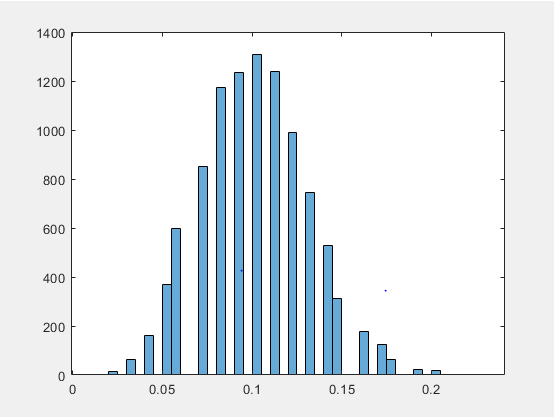
\includegraphics{2.png}


\end{document}
